% CA6127 group project technical review — GLIGEN vs MIGC
% Build: cd report && pdflatex report && pdflatex report
\documentclass[10pt,twocolumn]{article}
\usepackage[a4paper,margin=1.9cm,columnsep=0.7cm]{geometry}
\usepackage{graphicx,booktabs,amsmath,multirow,xcolor}
\usepackage[expansion=false]{microtype}
\usepackage{placeins,float}
\renewcommand{\topfraction}{0.92}\renewcommand{\bottomfraction}{0.6}\renewcommand{\textfraction}{0.05}\renewcommand{\floatpagefraction}{0.85}\setcounter{topnumber}{3}\setcounter{totalnumber}{5}
\renewcommand{\dbltopfraction}{0.99}\setcounter{dbltopnumber}{3}
\usepackage[font=small,labelfont=bf,skip=4pt]{caption}
\usepackage[hidelinks]{hyperref}
\usepackage{enumitem}
\setlist{nosep,leftmargin=*}
\graphicspath{{figures/}}
% generated by analysis/make_report_tables.py -- do not edit
\newcommand{\AttrG}{0.321}
\newcommand{\AttrM}{0.665}
\newcommand{\AttrDelta}{+0.344}
\newcommand{\AttrDeltaCI}{[+0.294, +0.393]}
\newcommand{\AttrGap}{0.34}
\newcommand{\RecallG}{0.92}
\newcommand{\RecallM}{0.93}
\newcommand{\PosDelta}{+0.06}
\newcommand{\IoUDelta}{+0.05}
\newcommand{\ColPosG}{40\%}
\newcommand{\ColPosM}{76\%}
\newcommand{\ImgG}{0.065}
\newcommand{\ImgM}{0.280}
\newcommand{\IQADelta}{+0.018}
\newcommand{\LeakG}{28\%}
\newcommand{\LeakM}{9\%}
\newcommand{\ColWrongG}{49\%}
\newcommand{\ColWrongM}{21\%}
\newcommand{\MissG}{3\%}
\newcommand{\MissM}{1\%}
\newcommand{\MislocG}{16\%}
\newcommand{\MislocM}{12\%}
\newcommand{\LeakShareG}{57\%}
\newcommand{\LayoutsBetter}{85}
\newcommand{\LayoutsTotal}{100}
\newcommand{\InstPerImage}{4}
\newcommand{\InstPerMethod}{800}
\newcommand{\ConfYB}{31}
\newcommand{\ConfBrBl}{14}
\newcommand{\ConfYBl}{10}
\newcommand{\ConfThree}{55}
\newcommand{\ConfTotal}{166}
\newcommand{\ConfShare}{33\%}
\newcommand{\LvlTwoG}{0.53}
\newcommand{\LvlSixG}{0.28}
\newcommand{\LvlTwoM}{0.71}
\newcommand{\LvlSixM}{0.68}
\newcommand{\OvNoneM}{0.80}
\newcommand{\OvHighM}{0.53}
\newcommand{\OvNoneDelta}{+0.49}
\newcommand{\OvHighDelta}{+0.22}
\newcommand{\OvHighDeltaCI}{[+0.09, +0.35]}
\newcommand{\SameCatMaxChange}{0.05}
\newcommand{\SizeQoneG}{0.20}
\newcommand{\SizeQfourG}{0.38}
\newcommand{\SizeQoneM}{0.61}
\newcommand{\SizeQfourM}{0.65}
\newcommand{\ThrGLo}{0.18}
\newcommand{\ThrGHi}{0.41}
\newcommand{\ThrMLo}{0.45}
\newcommand{\ThrMHi}{0.76}
\newcommand{\ThrGapLo}{0.27}
\newcommand{\ThrGapHi}{0.36}
\newcommand{\ThrGapAllPositive}{never include zero}
\newcommand{\FtGoneFive}{+0.042}
\newcommand{\FtGtwoFive}{+0.050}
\newcommand{\FtMaxGain}{+0.05}
\newcommand{\FtMinGain}{+0.03}
\newcommand{\LrContrast}{+0.042 [$-$0.004, +0.093]}
\newcommand{\GoneGtwoContrast}{+0.008 [$-$0.029, +0.045]}
\newcommand{\GoneFiveHundred}{0.321}
\newcommand{\GoneTwoThousand}{0.304}
\newcommand{\ColPosValG}{0.31}
\newcommand{\ColPosValLo}{0.34}
\newcommand{\ColPosValHi}{0.38}
\newcommand{\LeakValG}{0.36}
\newcommand{\LeakValGtwo}{0.30}
\newcommand{\LeakValCI}{[$-$0.10, $-$0.01]}
\newcommand{\RecallValG}{0.95}
\newcommand{\ValImages}{50}
\newcommand{\PosNetDrift}{2.7}
\newcommand{\GateMaxChange}{0.005}
\newcommand{\GateMaxAbs}{0.06}
\newcommand{\GligenSteps}{15}
\newcommand{\MigcSteps}{25}
\newcommand{\PosNetParamsM}{1.08}
\newcommand{\FuserParamsM}{208}
\newcommand{\FuserFrac}{19.5\%}
\newcommand{\GligenAddedM}{209}
\newcommand{\GligenAddedFrac}{19.6\%}
\newcommand{\PosNetFrac}{0.10\%}
\newcommand{\MigcParamsM}{57.4}
\newcommand{\MigcFrac}{6.7\%}
\newcommand{\SdUnetM}{860}
\newcommand{\FuserCount}{16}
\newcommand{\SecG}{5.7}
\newcommand{\MemG}{9.4}
\newcommand{\SecM}{6.5}
\newcommand{\MemM}{7.8}
\newcommand{\TrainMemGone}{5.8}
\newcommand{\TrainMemGtwo}{8.4}
\newcommand{\ParamRatio}{193}
   % every result number quoted below; generated by analysis/make_report_tables.py
\newcommand{\G}{GLIGEN}
\newcommand{\M}{MIGC}
% ---- data-status switch: set to {} once the cluster results are committed and figures regenerated
\newcommand{\datastatus}{\footnote{Numbers are computed from the test-set run committed in the repository; its metadata indicates a local RTX~4070 run, but no explicit \texttt{provenance.json} confirms the machine and run owner, so the result is provisional. Earlier group notes mention an A40 result, but its raw files are absent and it is not used here; see \texttt{outputs/final\_analysis/PROVENANCE.md}.}}

\title{\vspace{-1.2em}\Large\textbf{Where Does Layout-to-Image Control Break?\\ A Controlled Comparison of GLIGEN and MIGC on COCO-MIG}\vspace{-0.3em}}
\author{Group XX: [names as on student cards] \\ CA6127 Transformer and Generative Adversarial Networks, NTU}
\date{\vspace{-1.5em}}

\begin{document}
\maketitle

\begin{abstract}
We study \emph{multi-instance controllable generation}: given a caption and a set of (phrase, bounding box) pairs such as ``a red donut'' at a given location, the model must place every object in its box with the requested attribute. We compare two representative methods built on the same Stable Diffusion~1.4 backbone---GLIGEN, which injects box tokens through gated self-attention in all 16 transformer blocks, and MIGC, which replaces cross-attention in four low-resolution layers by a divide-and-conquer instance controller (Enhancement Attention, Layout Attention, Shading Aggregation Controller). We re-implement the MIG-Bench evaluation (Grounding~DINO + SAM + HSV colour test), fix every shared generation setting, and evaluate 100 COCO-MIG layouts~$\times$~2 seeds with layout-level bootstrap confidence intervals and paired comparisons. Both methods draw the requested objects equally often (Object Recall \RecallG{} vs \RecallM), but MIGC's instance success is twice GLIGEN's (\AttrM{} vs \AttrG); the gap is accompanied almost entirely by colour errors, and GLIGEN renders another instance's colour in \LeakG{} of all cases. The most plausible explanation is the architectural difference (shared attention vs isolated instance branches), which we argue from the mechanism and from the failure profiles but have not isolated with a single-component ablation. We show that the ranking is stable under the evaluator's colour threshold, that GLIGEN degrades with object count while MIGC degrades with box overlap, and that fine-tuning GLIGEN's grounding modules on 3\,000 COCO images gives at most a small gain in colour binding (\FtMinGain--\FtMaxGain{} on a 30-layout validation set, intervals near zero) without changing localisation. Code and all result tables are in the submitted package.
\end{abstract}

\section{Introduction}
Text-to-image diffusion models follow a prompt well but ignore \emph{where} things go and frequently mix up attributes when several objects are requested. Layout-to-image (L2I) generation adds a set of bounding boxes with per-box phrases as an extra condition, which makes the task testable: an evaluator can check whether each box contains the requested object with the requested attribute. The multi-instance version of this task (MIG) is hard because the conditions interact---two instances of the same category with different colours, overlapping boxes, or six objects in one image all stress the mechanism that routes each phrase to its region.

We selected two methods that make opposite design choices while sharing the same frozen backbone (SD~1.4), so that differences are more likely to come from the control mechanism than from the generator:
\begin{itemize}
\item \textbf{GLIGEN}~\cite{gligen} (CVPR~2023) encodes each (phrase, box) pair as a grounding token and lets image tokens attend to all grounding tokens through a new \emph{gated self-attention} layer in every transformer block.
\item \textbf{MIGC}~\cite{migc} (CVPR~2024) processes every instance in its \emph{own} masked cross-attention branch and merges the branches with a learned per-pixel controller; it introduced the COCO-MIG benchmark we use.
\end{itemize}
Our contributions are a controlled and fully reproducible comparison (Sec.~\ref{sec:setup}), a decomposition of the gap into localisation vs.\ attribute binding and a failure-mode analysis by difficulty condition (Sec.~\ref{sec:results}), an evaluator sensitivity study (Sec.~\ref{sec:sens}), an analysis of the key components with real tensor shapes (Sec.~\ref{sec:arch}), and a hyper-parameter study of fine-tuning GLIGEN's grounding modules (Sec.~\ref{sec:ft}).

\section{Methods}\label{sec:arch}
Both methods keep the SD~1.4 UNet (\SdUnetM\,M parameters) frozen and add trainable modules; Figure~\ref{fig:arch} shows where. All shapes below were recorded with forward hooks on a real 2-object sample (\texttt{outputs/analysis/*\_probe.json}).

\begin{figure*}[t]
\centering
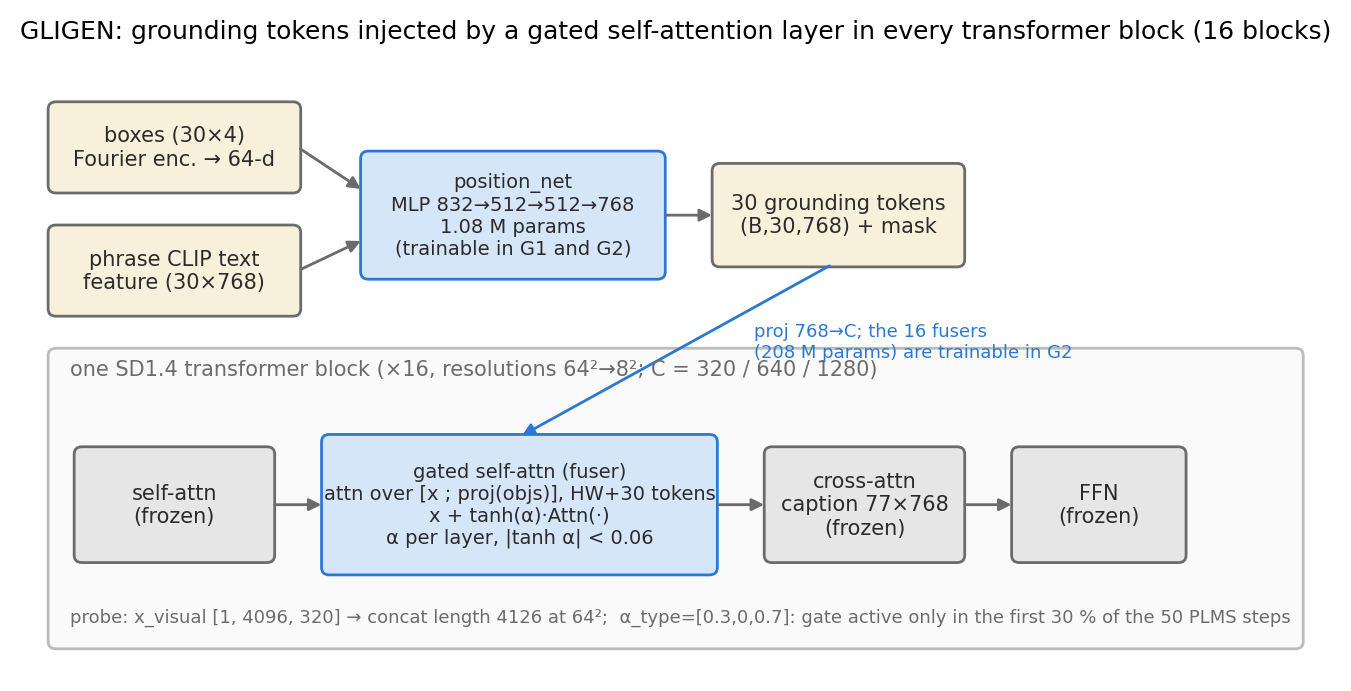
\includegraphics[width=0.72\textwidth]{arch_gligen.png}\\[2pt]
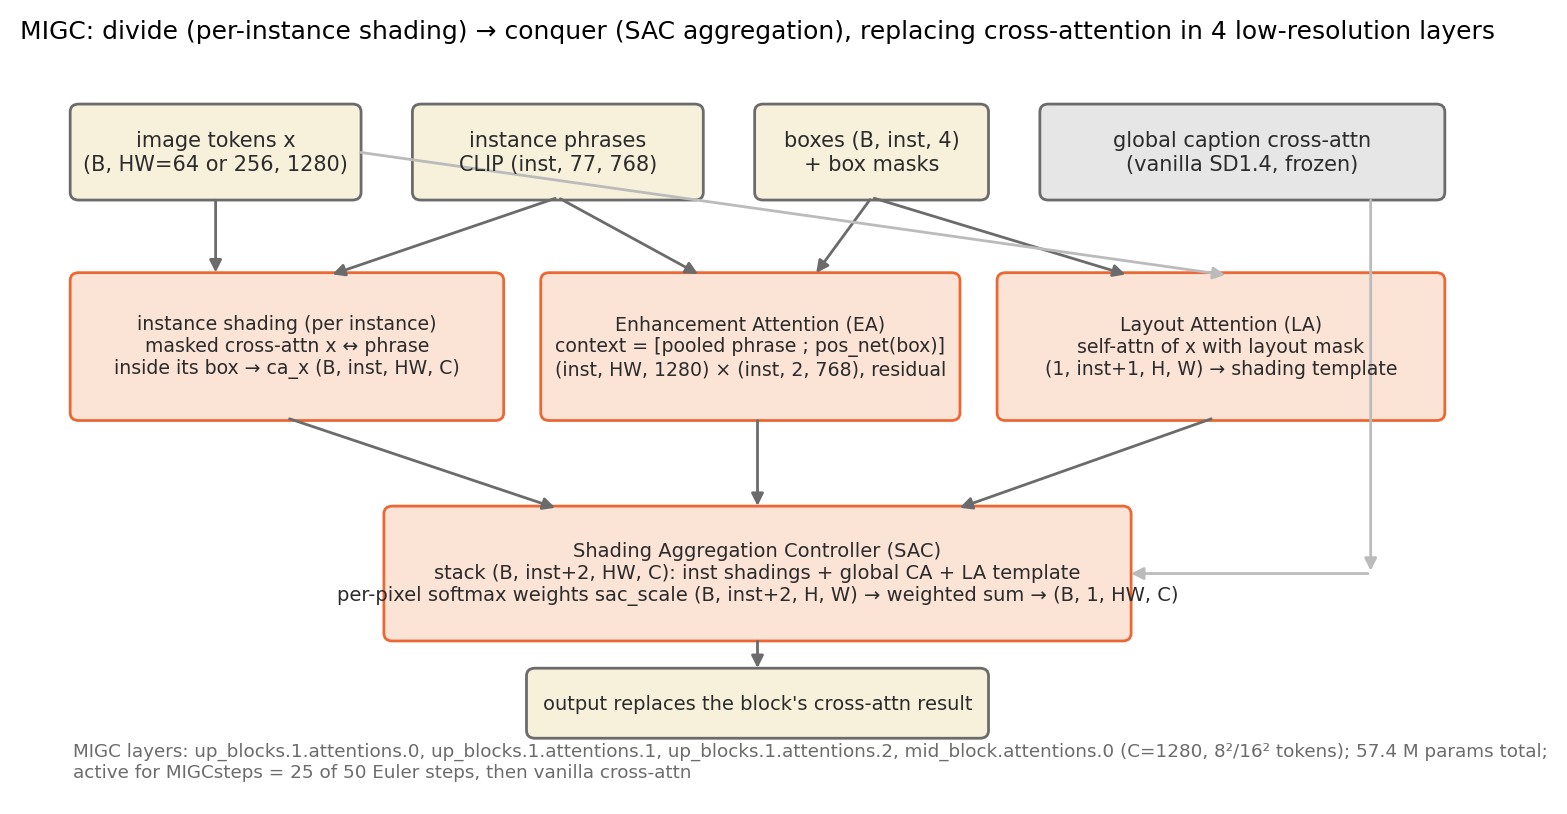
\includegraphics[width=0.72\textwidth]{arch_migc.png}
\caption{Control paths. \textbf{Top:} GLIGEN inserts a gated self-attention (``fuser'') in all 16 transformer blocks; grounding tokens come from \texttt{position\_net}. \textbf{Bottom:} MIGC replaces cross-attention in 4 low-resolution layers; each instance is shaded in its own branch and the branches are merged by SAC. Shapes from our probes.}
\label{fig:arch}
\end{figure*}

\paragraph{GLIGEN.} The Fourier-encoded box (64-d) is concatenated with the CLIP text feature of its phrase (768-d) and mapped by a 3-layer MLP (832$\to$512$\to$512$\to$768) to a grounding token; 30 slots are always filled, empty ones with a learned null token (\PosNetParamsM\,M parameters). In each block, after the frozen self-attention, the $HW$ visual tokens are concatenated with the 30 projected grounding tokens (4\,126 tokens at $64^2$) and passed through a new self-attention whose visual part is added back with a per-layer scalar gate: $x \leftarrow x + \tanh(\alpha)\,\mathrm{Attn}([x;\,\mathrm{objs}])$. The \FuserCount{} fusers hold \FuserParamsM\,M parameters (\FuserFrac{} of the UNet). In the official checkpoint $|\tanh\alpha|<\GateMaxAbs$ in every layer. At inference the gate is only open during the first 30\% of the sampling steps (\GligenSteps{} of 50; \texttt{alpha\_type}=[0.3,0,0.7]). Nothing in this design ties the \emph{colour word} of a phrase to its box: the phrase is encoded as a whole, and the global caption---which contains all colour words---is still processed by the frozen cross-attention.

\paragraph{MIGC.} Only \texttt{mid\_block} ($8^2$) and the three \texttt{up\_blocks.1} attentions ($16^2$), all with $C{=}1280$, are replaced (\MigcParamsM\,M parameters, \MigcFrac). For every instance a masked cross-attention between the image tokens and that instance's phrase is computed inside its box, giving \texttt{ca\_x} of shape $(B,1{+}\text{inst},HW,C)$ where the extra slice is the ordinary caption cross-attention. \emph{Enhancement Attention} (EA) re-attends each instance to a 2-token context (pooled phrase + a box token from a small position net) to strengthen the response inside the box. \emph{Layout Attention} (LA) runs self-attention over image tokens with a layout mask $(1,\text{inst}{+}1,H,W)$ and yields a shading template shared by all instances. The \emph{Shading Aggregation Controller} (SAC) stacks the inst{+}2 candidates and predicts per-pixel softmax weights $(B,\text{inst}{+}2,H,W)$ with which they are blended, so the contribution of each instance to a pixel is an explicit, learned weighting. MIGC is active for the first \MigcSteps{} of 50 Euler steps.

\paragraph{Difference in one sentence.} GLIGEN lets all grounding tokens see each other inside one attention and relies on the frozen caption attention for appearance; MIGC isolates the instances until a learned arbiter merges them. Table~\ref{tab:diff} summarises the implementation facts.

\begin{table}[t]
\centering\small
\caption{Implementation facts (from official code and our probes).}
\label{tab:diff}
\footnotesize\setlength{\tabcolsep}{3pt}
\begin{tabular}{@{}lll@{}}
\toprule
 & GLIGEN & MIGC \\ \midrule
Injection & 30 tokens, self-attn & per-instance CA \\
Layers & 16 blocks, $64^2$--$8^2$ & 4 layers, $16^2$/$8^2$ \\
Spatial constraint & implicit & explicit mask + SAC \\
Isolation & none & until SAC \\
Added params & \GligenAddedM\,M (\GligenAddedFrac) & \MigcParamsM\,M (\MigcFrac) \\
Control steps & \GligenSteps/50 (30\%) & \MigcSteps/50 (50\%) \\
Official sampler & PLMS & Euler \\
s/img, GB (4070) & \SecG, \MemG & \SecM, \MemM \\ \bottomrule
\end{tabular}
\end{table}

\section{Experimental setup}\label{sec:setup}
\paragraph{Dataset.} COCO-MIG~\cite{migc} provides 800 layouts derived from COCO~val2014 boxes, each object given one of 7 colours (red, blue, green, yellow, black, white, brown) and 2--6 objects per image (levels L2--L6). We stratify by level into a \textbf{test} set of 100 layouts (20 per level), a \textbf{validation} set of 30 (used only for hyper-parameter choices) and a 10-layout pilot subset; the splits are disjoint and fixed (\texttt{manifests/}, sha256 recorded). The fine-tuning images come from COCO train2014, which is disjoint from the val2014 images that COCO-MIG layouts were derived from; because the bench file does not record COCO image IDs, we could verify source isolation and the absence of near-duplicate layouts (0 of 130 evaluation layouts match any training image at mean IoU $\geq0.9$) but could not check image IDs one by one. Every layout is generated with two seeds (42, 2025), so each method produces 200 test images containing 800 target instances. From the inputs alone we annotate each instance with difficulty conditions: same category with a different colour present (57\%), box overlap bucket by max IoU with another box (none/low$<$0.1/mid$<$0.3/high), and relative size quartile. COCO-MIG contains no COCO-``small'' objects (minimum side 66\,px at $512^2$), so size is analysed by quartile.

\paragraph{Unified generation settings.} $512{\times}512$, 50 steps, CFG 7.5, the same negative prompt, and the same initial noise for a given seed, fp16 autocast with fp32 weights. Both adapters were verified to reproduce the official inference scripts pixel-for-pixel; GLIGEN's attention was switched to SDPA with a maximum $\epsilon$ error of $7.9{\times}10^{-4}$. Two settings were deliberately left at each method's official value and therefore differ: the sampler (PLMS in GLIGEN's ldm code, Euler in MIGC's diffusers code) and the number of steps during which layout control is active (GLIGEN \GligenSteps/50, MIGC \MigcSteps/50). Both are discussed in Sec.~\ref{sec:limits}; the control duration is also varied on the validation set in Sec.~\ref{sec:ft}.

\paragraph{Evaluation.} We re-implemented the MIG-Bench protocol: Grounding~DINO (SwinT-OGC, box/text threshold 0.25) detects the category; \emph{Position Success} = max IoU with a same-category detection $\geq0.5$; SAM, prompted with the ground-truth box, segments the object; \emph{Attribute Success} (= MIG-Bench instance success) additionally requires that $\geq20\%$ of the mask pixels fall in the HSV range of the target colour; \emph{Image Success} requires all instances to succeed; \emph{official mIoU} zeroes the IoU of colour-wrong instances. We add diagnostics that are reported under separate names: \emph{Object Recall} (a one-to-one Hungarian match exists), \emph{Localisation IoU} (colour ignored), the exclusive failure type (missing / mislocated / colour-wrong) and \emph{Color Leakage Rate}---the dominant mask colour is another instance's target colour. Image quality is measured with CLIP-IQA. All intervals are 95\% percentile bootstraps over \emph{layouts} (both seeds and all objects of a layout resampled together, 5\,000 draws); method differences are paired on identical (layout, seed, object).

\section{Results and analysis}\label{sec:results}

\subsection{Overall comparison}
\begin{table*}[t]
\centering\small
\caption{Test set, 100 layouts $\times$ 2 seeds (800 instances per method). 95\% layout-bootstrap CIs; the last column is the paired difference.}
\label{tab:main}
\small\setlength{\tabcolsep}{6pt}
\begin{tabular}{@{}lrrl@{}}
\toprule
Metric & GLIGEN & MIGC & MIGC $-$ GLIGEN \\ \midrule
Object Recall $\uparrow$ & 0.917 & 0.932 & +0.015 [$-$0.012, +0.042] \\
Position Success $\uparrow$ & 0.809 & 0.873 & +0.064 [+0.027, +0.102] \\
Localisation IoU $\uparrow$ & 0.690 & 0.741 & +0.051 [+0.023, +0.080] \\
\textbf{Attribute Success} $\uparrow$ & 0.321 & 0.665 & \textbf{+0.344 [+0.294, +0.393]} \\
~~given position OK & 0.397 & 0.762 & +0.365 (unpaired) \\
Official mIoU $\uparrow$ & 0.288 & 0.572 & +0.284 [+0.243, +0.325] \\
Image Success $\uparrow$ & 0.065 & 0.280 & +0.215 [+0.150, +0.280] \\
Color Leakage Rate $\downarrow$ & 0.279 & 0.091 & $-$0.188 [$-$0.229, $-$0.142] \\
Missing Rate $\downarrow$ & 0.033 & 0.009 & $-$0.024 [$-$0.042, $-$0.006] \\
Mislocation Rate $\downarrow$ & 0.159 & 0.119 & $-$0.040 [$-$0.078, $-$0.005] \\
CLIP-IQA $\uparrow$ & 0.689 & 0.707 & +0.018 [+0.002, +0.034] \\
\bottomrule%

\end{tabular}
\end{table*}

\begin{figure*}[t]
\centering
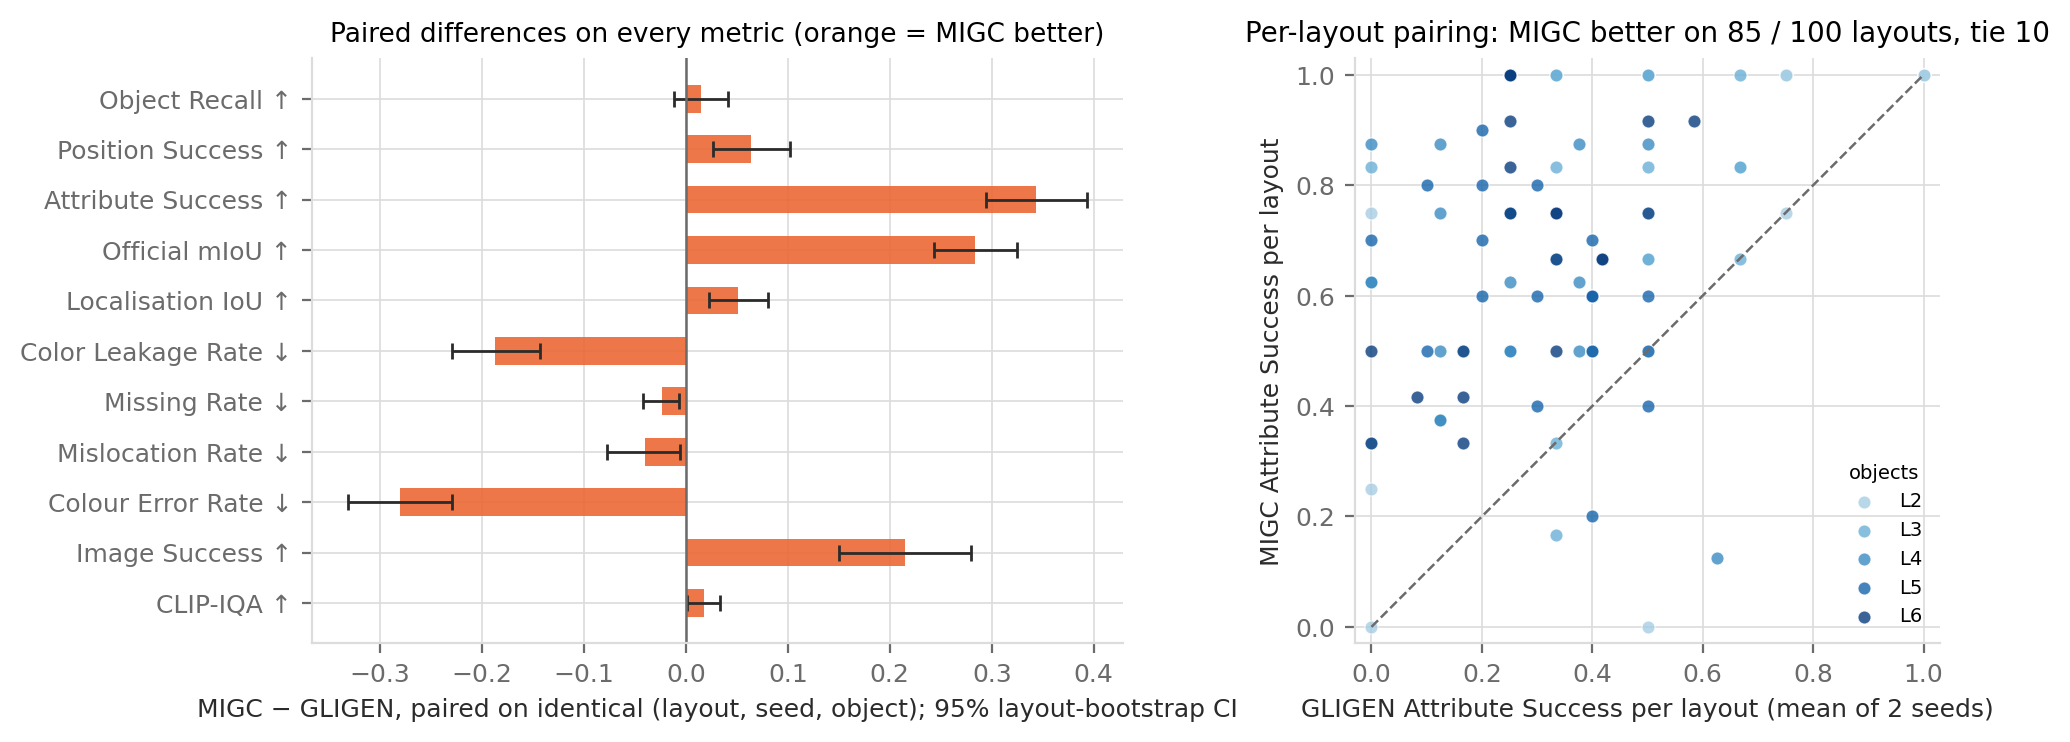
\includegraphics[width=0.92\textwidth]{test_paired.png}
\caption{\textbf{Left:} paired MIGC$-$GLIGEN difference for every metric with 95\% layout-bootstrap CI (bar colour: orange = MIGC better). \textbf{Right:} per-layout Attribute Success; MIGC is better on \LayoutsBetter{} of \LayoutsTotal{} layouts and never worse on a whole level.}
\label{fig:paired}
\end{figure*}

Table~\ref{tab:main} and Figure~\ref{fig:paired} give the headline result.\datastatus{} Three observations structure the rest of the analysis. (i)~\textbf{Both methods draw the objects.} Object Recall is \RecallG{} vs \RecallM{} and the difference is not significant; MIGC localises slightly better (\PosDelta{} Position Success, \IoUDelta{} IoU). (ii)~\textbf{The gap goes with attribute binding.} Among instances that are in the right place, \ColPosG{} of GLIGEN's have the right colour versus \ColPosM{} of MIGC's. The \AttrGap{} gap in Attribute Success is thus accompanied mainly by a difference in colour pass rate while position differences are small; we have not performed a causal decomposition, because an instance is counted as a colour failure only once it has passed the position test. (iii)~\textbf{Image-level success amplifies instance-level differences} (\InstPerImage{} instances per image on average): \ImgG{} vs \ImgM. Image quality is essentially unchanged (CLIP-IQA \IQADelta), so MIGC's control is not bought with fidelity.

\subsection{Failure modes}
\begin{figure*}[t]
\centering
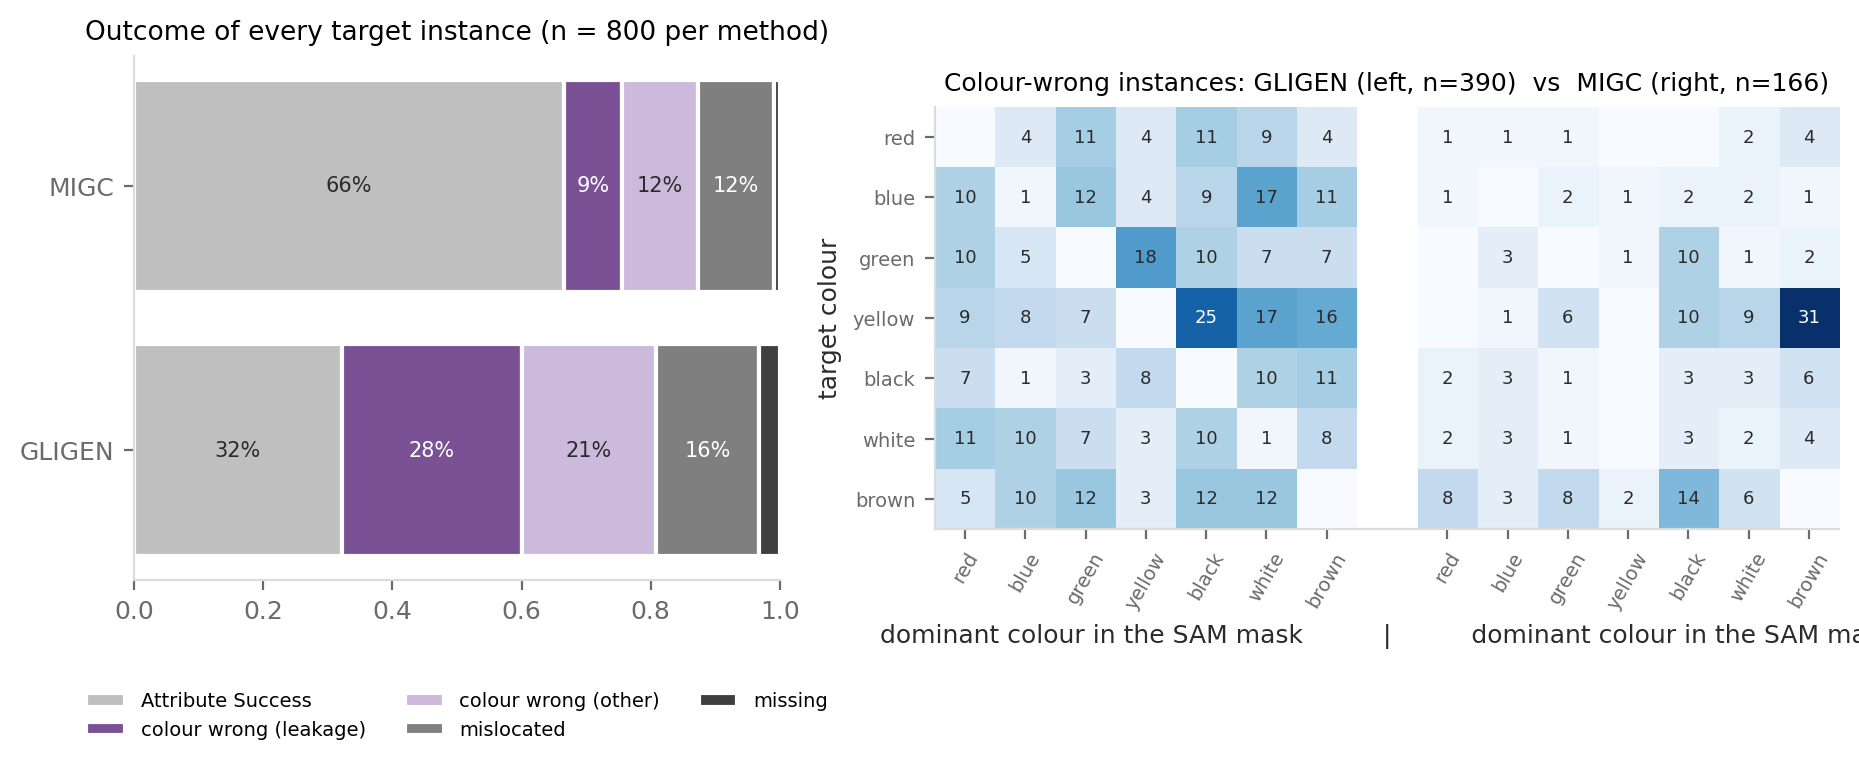
\includegraphics[width=0.92\textwidth]{test_failure_modes.png}
\caption{\textbf{Left:} every target instance falls in exactly one outcome. GLIGEN's colour errors split into leakage (another instance's colour) and other. \textbf{Right:} target vs dominant colour for colour-wrong instances: GLIGEN's confusions are diffuse, MIGC's concentrate on yellow$\to$brown and brown$\to$black.}
\label{fig:fail}
\end{figure*}

Figure~\ref{fig:fail} decomposes failures. GLIGEN: \ColWrongG{} of instances are colour-wrong, and \LeakShareG{} of those are \emph{leakage}---the mask is dominated by a colour requested for a \emph{different} instance; the confusion matrix is almost uniform. This is consistent with the architecture: the grounding tokens share one attention and the colours are rendered by the frozen caption cross-attention, which sees ``a red donut and a green donut and \dots'' with no mechanism tying ``red'' to a box. MIGC: \ColWrongM{} colour-wrong, \LeakM{} leakage, and \ConfShare{} of its colour errors (\ConfThree{} of \ConfTotal) fall on three HSV-adjacent pairs (yellow$\to$brown \ConfYB, brown$\to$black \ConfBrBl, yellow$\to$black \ConfYBl). Visual inspection (Figure~\ref{fig:cases}, category E) shows tan cows judged ``brown'' and clearly brown vases judged ``red'': part of MIGC's residual error is the evaluator's colour table, not the model. Missing and mislocated objects are rare for both (GLIGEN \MissG/\MislocG, MIGC \MissM/\MislocM); several GLIGEN mislocations are objects that extend beyond their box, which could be related to the 70\% of steps in which the gate is closed, although we did not test this.

\begin{figure*}[t]
\centering
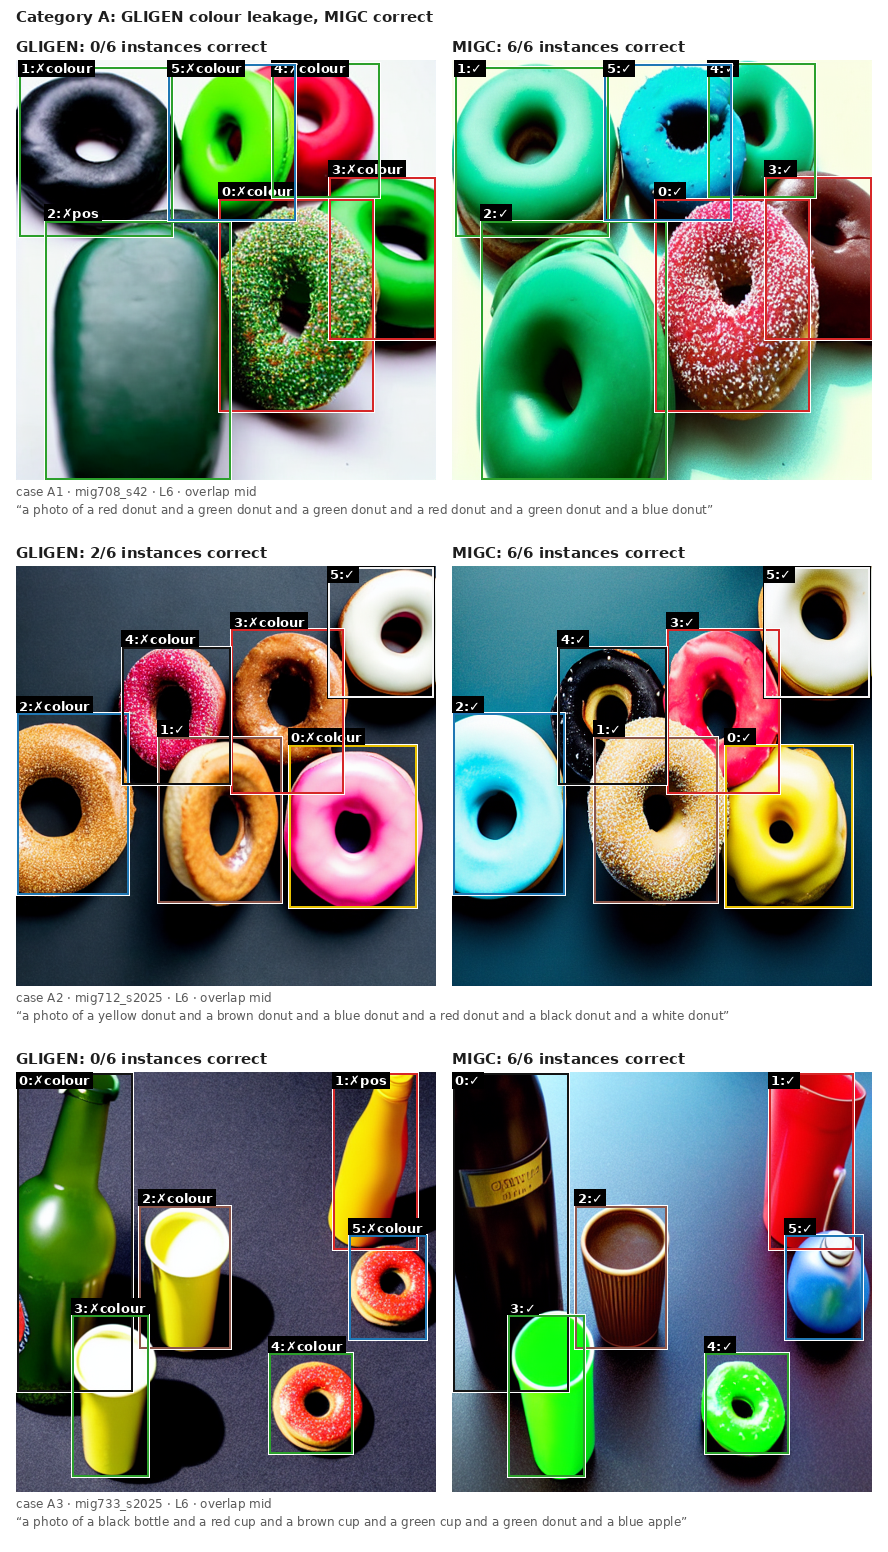
\includegraphics[width=0.42\textwidth]{cases_A.png}\hfill
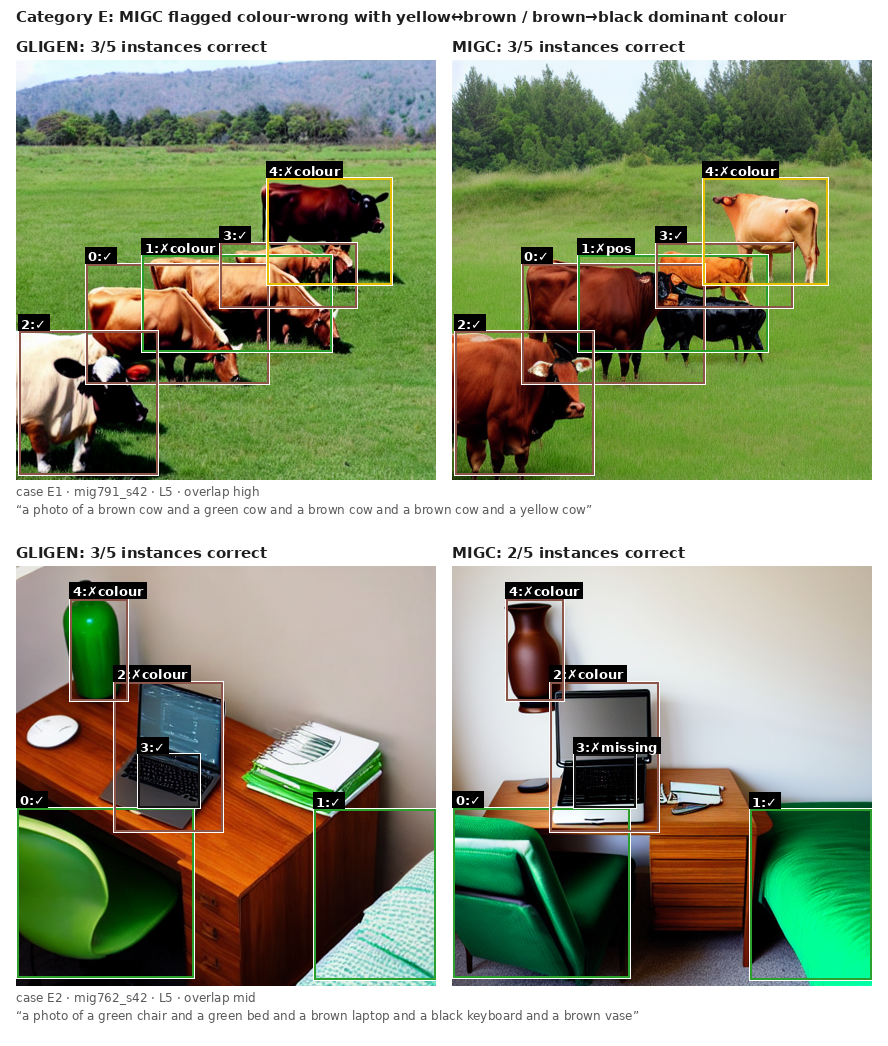
\includegraphics[width=0.42\textwidth]{cases_E.png}
\caption{Qualitative cases selected by fixed rules (\texttt{analysis/failure\_cases.py}); boxes show the target layout in the target colour, labels the evaluator verdict. \textbf{Left (A):} GLIGEN colour leakage on 6-object layouts where MIGC is fully correct. \textbf{Right (E):} MIGC instances judged colour-wrong on yellow/brown boundaries. Categories B--D (GLIGEN misses, MIGC fails, both fail under overlap) are in the package.}
\label{fig:cases}
\end{figure*}

\subsection{Difficulty conditions}
\begin{figure*}[t]
\centering
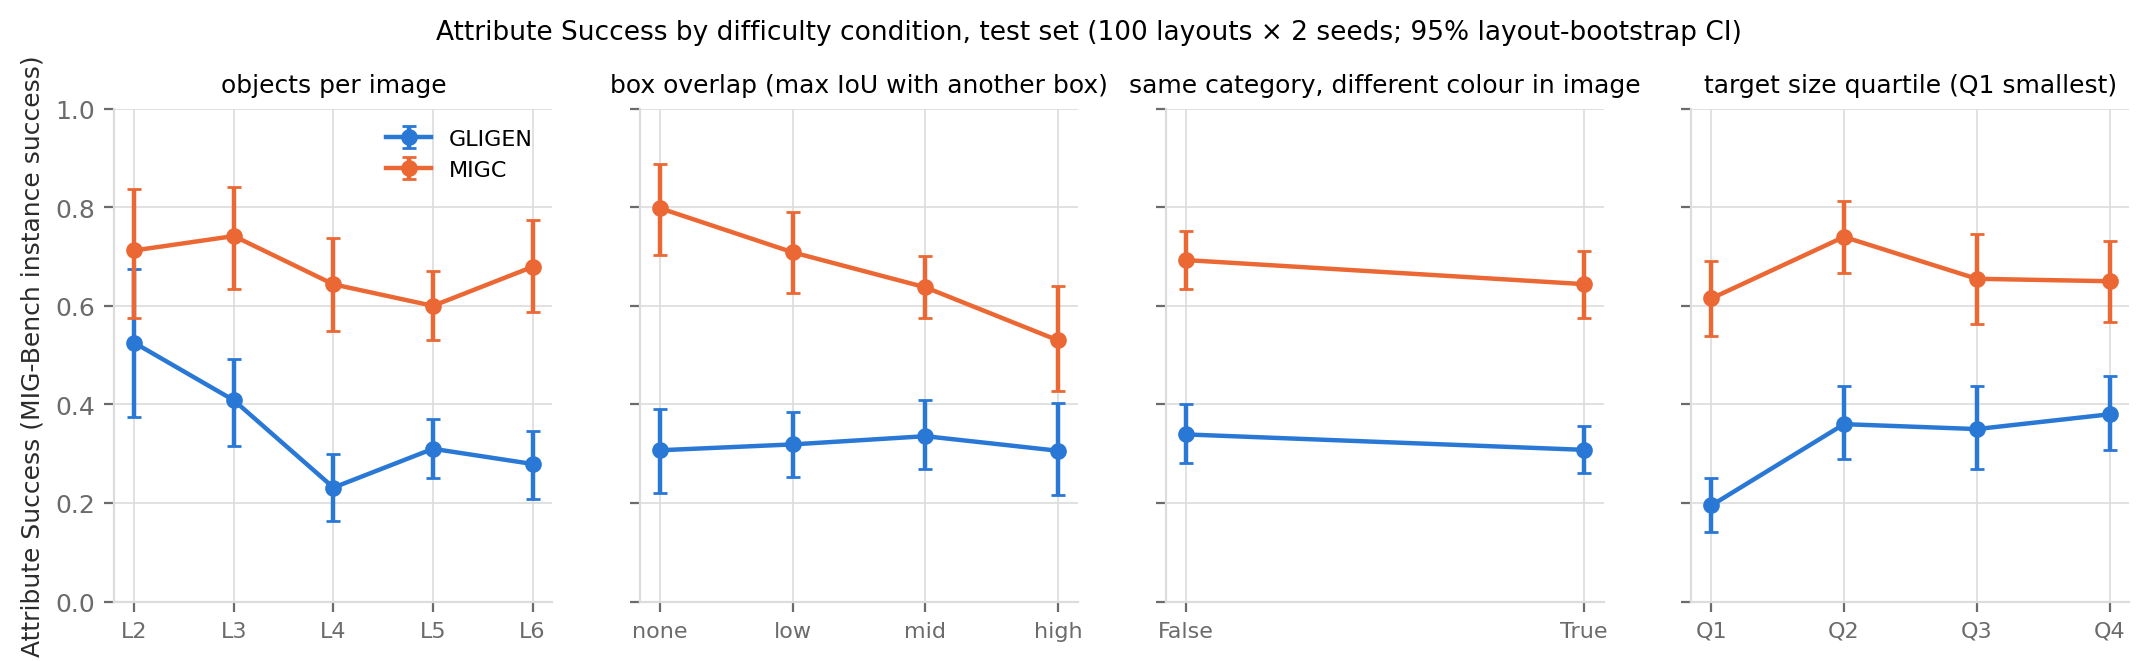
\includegraphics[width=0.95\textwidth]{test_subgroups.png}
\caption{Attribute Success by difficulty condition (95\% layout-bootstrap CIs). GLIGEN degrades with object count and small targets; MIGC degrades with box overlap; neither is affected by same-category-different-colour beyond its baseline.}
\label{fig:sub}
\end{figure*}

Figure~\ref{fig:sub} separates the conditions. \textbf{Object count} is GLIGEN's main difficulty (\LvlTwoG{} at L2 $\to$ \LvlSixG{} at L6) while MIGC is flat (\LvlTwoM{} $\to$ \LvlSixM): a plausible reading is that more instances mean more colour words competing in one shared attention, whereas MIGC's branches do not see each other. \textbf{Box overlap} is MIGC's main difficulty: \OvNoneM{} with no overlap $\to$ \OvHighM{} with high overlap, so the gap narrows from \OvNoneDelta{} to \OvHighDelta{} \OvHighDeltaCI. This contradicts our prior expectation that the SAC blending would help under overlap. One reading, not tested here, is that in an overlapping region two instance branches each shade the pixels with their own colour and the learned weighted blend dilutes both, so one of them falls below the 20\% colour threshold. GLIGEN is flat here, possibly because it is already near its floor. \textbf{Same category, different colour} changes neither method by more than \SameCatMaxChange: colour errors are not specifically same-category confusions. \textbf{Small targets} (smallest quartile, normalised area $<0.051$) hurt GLIGEN strongly (\SizeQoneG{} vs \SizeQfourG{} for the largest quartile) but not MIGC (\SizeQoneM{} vs \SizeQfourM), even though MIGC controls only at $8^2$/$16^2$, where a smallest-quartile box covers only about 4--13 of the 256 tokens at $16^2$ (1--3 at $8^2$). This suggests that how instances are isolated matters more than the resolution at which control is applied.

\begin{figure*}[!t]
\centering
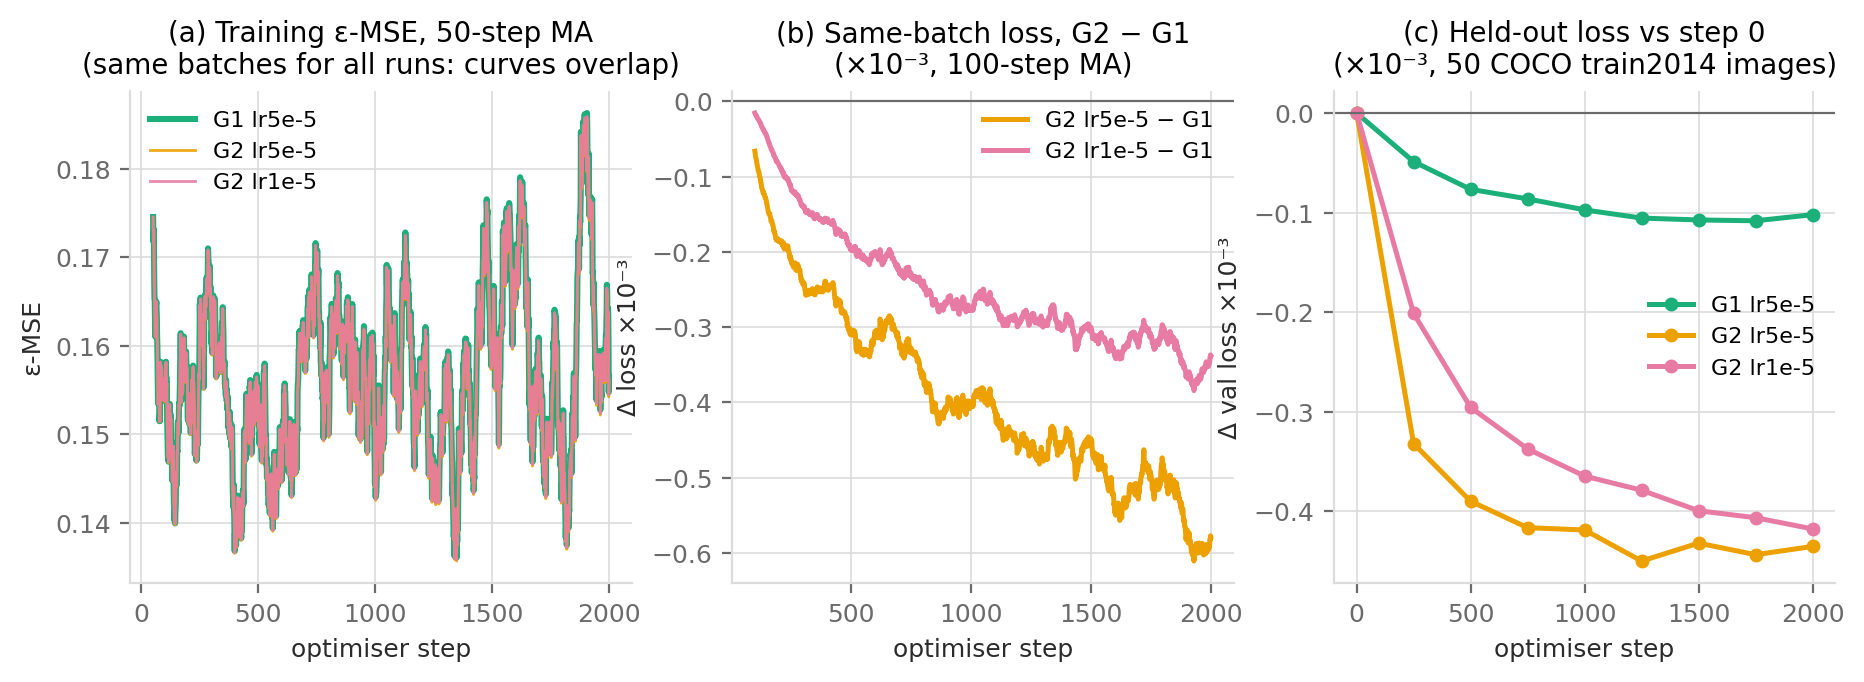
\includegraphics[width=0.9\textwidth]{train_curves.png}
\caption{Training. (a)~All runs see identical batches, so training-loss curves overlap; (b)~the same-batch difference shows G2 fits better than G1; (c)~held-out loss on \ValImages{} COCO images saturates after $\sim$1\,250 steps. Absolute changes are $<0.3\%$---expected with frozen SD and no attribute supervision.}
\label{fig:train}
\end{figure*}
\subsection{Evaluator sensitivity}\label{sec:sens}
\begin{figure}[t]
\centering
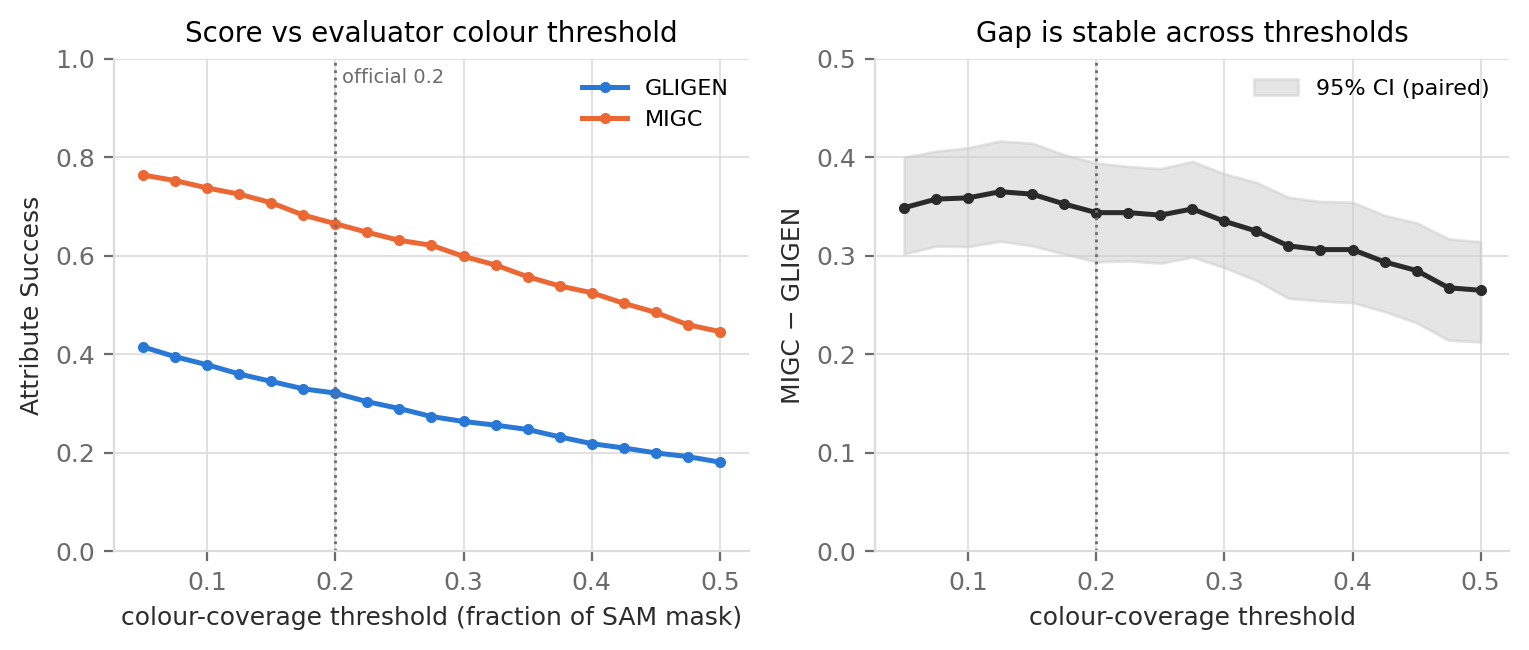
\includegraphics[width=\linewidth]{test_colour_threshold.png}
\caption{Sweeping the colour-coverage threshold of the evaluator (images, detections and masks fixed). Scores move, the gap does not.}
\label{fig:thr}
\end{figure}
Because the headline metric depends on a hand-set threshold (20\% of mask pixels in the target HSV range), we recomputed Attribute Success from the cached per-instance colour ratios for thresholds 0.05--0.5 (Figure~\ref{fig:thr}). Absolute scores fall almost linearly (GLIGEN \ThrGHi$\to$\ThrGLo, MIGC \ThrMHi$\to$\ThrMLo) but the paired gap stays within \ThrGapLo--\ThrGapHi{} with intervals that \ThrGapAllPositive. The ranking is therefore robust; the absolute numbers are not and must always be reported with the threshold. The cache cannot be used to vary the position threshold (colour is only measured for position-correct instances) or to swap the detector---those require new GPU evaluation.

\subsection{Fine-tuning GLIGEN's grounding modules}\label{sec:ft}
GLIGEN's weakness is binding, so we asked whether the two modules that carry the layout signal can be adapted cheaply. We fine-tuned, from the official checkpoint, (G1) only \texttt{position\_net} (\PosNetParamsM\,M parameters, \PosNetFrac) and (G2) \texttt{position\_net}+fusers (\GligenAddedM\,M, \GligenAddedFrac) on 3\,000 COCO train2014 images with category-name phrases only (no colour supervision; source-isolated from the val2014-derived test layouts and checked for near-duplicate layouts as described in Sec.~\ref{sec:setup}). Shared settings: 2\,000 steps, effective batch 8, AdamW without weight decay, 100 warm-up steps then constant LR, bf16, the official $\epsilon$-MSE objective with 10\% grounding dropout, optimiser state reset; checkpoints at 500 and 2\,000 steps; G2 at LR $5{\times}10^{-5}$ and $10^{-5}$. All weight and gradient checks passed (frozen parameters unchanged, every trainable parameter updated).


\begin{table*}[t]
\centering\small
\caption{Fine-tuned GLIGEN on the validation set (30 layouts $\times$ 2 seeds, grounding ratio $r{=}0.5$). Paired difference vs the official checkpoint. Exploratory: 30 layouts only.}
\label{tab:ft}
\setlength{\tabcolsep}{3pt}
\begin{tabular}{@{}lrlrr@{}}
\toprule
Run & Attr.\ Succ. & $\Delta$ vs official [CI] & Col.$|$Pos & Loc.\ IoU \\ \midrule
official & 0.279 & -- & 0.310 & 0.746 \\
G1 5e-5 @500 & 0.321 & \textbf{+0.042 [+0.004, +0.080]} & 0.363 & 0.747 \\
G1 5e-5 @2000 & 0.304 & +0.025 [$-$0.012, +0.064] & 0.340 & 0.755 \\
G2 1e-5 @500 & 0.287 & +0.008 [$-$0.032, +0.047] & 0.322 & 0.753 \\
G2 1e-5 @2000 & 0.296 & +0.017 [$-$0.028, +0.065] & 0.327 & 0.764 \\
G2 5e-5 @500 & 0.329 & \textbf{+0.050 [+0.009, +0.096]} & 0.369 & 0.751 \\
G2 5e-5 @2000 & 0.325 & +0.046 [$-$0.016, +0.111] & 0.375 & 0.737 \\
\bottomrule%

\end{tabular}
\end{table*}

\paragraph{Hyper-parameters (Table~\ref{tab:ft}, Figure~\ref{fig:train}).} \emph{Learning rate:} at $10^{-5}$ G2 is indistinguishable from the official model; at $5{\times}10^{-5}$ the validation point estimates are higher, but the direct contrast (G2 5e-5 vs 1e-5 at 500 steps: \LrContrast) includes zero, so the data do not establish that 5e-5 is better---only that 1e-5 showed no measurable effect. \emph{Checkpoint:} we found no consistent advantage of 2\,000 over 500 steps (G1 drops \GoneFiveHundred$\to$\GoneTwoThousand; all 2000$-$500 contrasts include zero), and held-out loss saturates by $\sim$1\,250 steps while weight drift keeps growing (position\_net $\|\Delta\theta\|_2$ reaches \PosNetDrift). We did not evaluate intermediate checkpoints on the task, so we cannot say where between 500 and 2\,000 steps the plateau begins. \emph{Grounding ratio:} the group's Stage C-1 log (README \S4.3) reports that extending GLIGEN's gate from 30\% to 50\% of the steps gave a small, significant gain in validation Localisation IoU and a smaller, non-significant change in Attribute Success, and that MIGC improved mildly with longer control. The raw outputs of that experiment are not in the code package, so we quote no figures from it here and treat it as unverified; all fine-tuned runs use $r{=}0.5$, the value chosen from that log.

\paragraph{Where the change appears.} The largest point-estimate changes are in colour-given-position (\ColPosValG$\to$\ColPosValLo--\ColPosValHi) and leakage (G2 5e-5 @500: \LeakValG$\to$\LeakValGtwo{} \LeakValCI). These validation results do not establish consistent gains in localisation or object presence. Training only \texttt{position\_net} gives a change of the same size as G2 (\FtGoneFive{} vs \FtGtwoFive, contrast \GoneGtwoContrast) with 1/\ParamRatio{} of the trainable parameters and \TrainMemGone{} vs \TrainMemGtwo\,GB. The per-layer gate values $\tanh\alpha$ barely move ($<\GateMaxChange$); the small gate changes do not establish whether the gates contributed, which would require a separate ablation. Any observed change could sit in the fuser weights, in \texttt{position\_net}, or in their interaction. With at most \FtMaxGain{} on validation and no colour supervision, this kind of fine-tuning is unlikely to close a \AttrGap{} gap; our hypothesis---untested---is that the binding problem sits in the frozen caption attention that the GLIGEN design leaves untouched.

\section{Discussion}\label{sec:limits}
\paragraph{Strengths and limitations of the methods.} GLIGEN is general (the same tokens can carry key-points or depth), touches every resolution and has an elegant train-time story (frozen SD, zero-initialised gates), but its shared-attention injection has no notion of instance ownership: attributes leak, and performance decays with instance count and small boxes. MIGC's per-instance branches give it strong binding at low cost (\MigcFrac{} extra parameters, 4 layers) and robustness to instance count, but the arbiter struggles when boxes overlap, its control exists only at $8^2$/$16^2$, and per-instance branches make inference time grow with the number of instances (Figure~\ref{fig:cost}).

\begin{figure}[H]
\centering
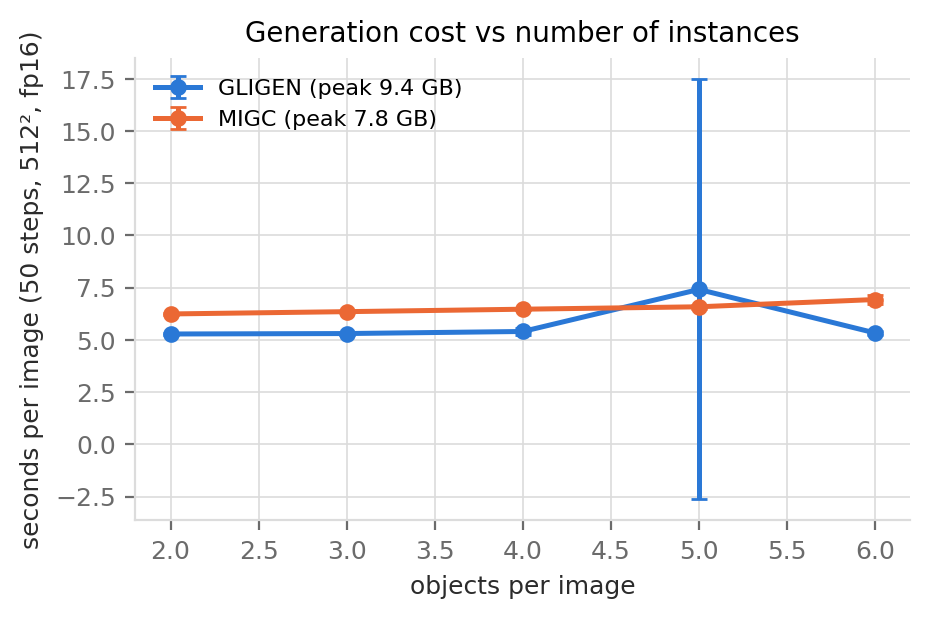
\includegraphics[width=0.72\linewidth]{test_cost.png}
\caption{Generation cost vs number of instances (RTX~4070, fp16, 50 steps). MIGC's time grows with instance count, GLIGEN's is constant (fixed 30 slots).}
\label{fig:cost}
\end{figure}

\paragraph{Limitations of this study.} (1)~No single-component ablation was run, so the architectural explanation of the gap is an interpretation supported by mechanism and failure profiles, not an isolated causal result. (2)~100 test layouts $\times$ 2 seeds; intervals are unadjusted for multiple comparisons and the validation set has only 30 layouts, so Sec.~\ref{sec:ft} is exploratory and several of its contrasts include zero. (3)~Two generation settings differ between the methods: the sampler (PLMS vs Euler, because the two official code bases do not share one) and the duration of layout control (\GligenSteps/50 vs \MigcSteps/50 steps). The group's (unverified) validation sweep suggests the duration changes GLIGEN's Attribute Success only slightly, but a part of the gap may be due to either setting and we cannot bound it without re-running both methods under one sampler and one schedule. (4)~Train/test isolation was verified at the source and layout level only; COCO image IDs are not available for the bench layouts. (5)~The HSV colour table misjudges yellow/brown/black boundaries, which penalises MIGC more. (6)~Fine-tuned models were evaluated on validation only; the test-set evaluation of the selected configurations (G1, G2 5e-5) is pending, and the grounding-ratio experiment is quoted qualitatively from the group log pending the raw files. (7)~Fine-tuning used category phrases only, so it tests adaptation of the grounding path, not attribute learning.

\paragraph{Future extensions.} The evidence is consistent with instance isolation being the decisive ingredient, but we have not isolated it. The first extension is therefore the missing ablation: (a)~adding an instance-mask constraint to GLIGEN's fuser (restrict each grounding token's attention to its box), which would test whether isolation alone fixes leakage without MIGC's extra branches; (b)~fine-tuning with colour-annotated phrases to separate ``cannot bind'' from ``never learned''; (c)~an overlap-aware aggregation for MIGC (soft ownership instead of softmax, or ordering by depth) targeting the one condition where it degrades; (d)~unifying the sampler (both code bases support DDIM) and extending to a second benchmark such as HRS or T2I-CompBench to check that the conclusions transfer.

\section{Conclusion}
On COCO-MIG with every shared setting fixed, GLIGEN and MIGC draw the requested objects equally often, but MIGC binds attributes to instances twice as reliably (\AttrM{} vs \AttrG), a ranking that survives changes to the evaluator threshold. The most plausible explanation is architectural---shared grounding attention versus isolated instance branches; it is consistent with the opposite difficulty profiles (GLIGEN fails with more objects, MIGC with overlapping boxes) and with the observation that cheaply adapting GLIGEN's grounding modules changes binding only marginally, but it has not been isolated by ablation. For practitioners: when per-instance attributes must be correct, prefer an instance-isolating controller; when boxes overlap heavily, neither method is reliable yet.

\begin{thebibliography}{9}\small
\bibitem{gligen} Y.~Li et al. GLIGEN: Open-Set Grounded Text-to-Image Generation. CVPR 2023.
\bibitem{migc} D.~Zhou et al. MIGC: Multi-Instance Generation Controller for Text-to-Image Synthesis. CVPR 2024.
\bibitem{sd} R.~Rombach et al. High-Resolution Image Synthesis with Latent Diffusion Models. CVPR 2022.
\bibitem{gdino} S.~Liu et al. Grounding DINO: Marrying DINO with Grounded Pre-Training for Open-Set Object Detection. ECCV 2024.
\bibitem{sam} A.~Kirillov et al. Segment Anything. ICCV 2023.
\bibitem{clipiqa} J.~Wang et al. Exploring CLIP for Assessing the Look and Feel of Images. AAAI 2023.
\end{thebibliography}

\section*{Reproducibility statement}
The submitted repository fixes the 100-layout test, 30-layout validation and 10-layout pilot manifests and records their hashes. From the repository root, \texttt{bash scripts/stageD\_analysis.sh} checks split and training-data isolation, recomputes the statistics, tables and figures from the committed per-instance records, verifies every reported number, and rebuilds the PDF when \texttt{pdflatex} is available. The CPU pipeline was independently rerun on an Apple Silicon Mac with Python~3.12 on 18~October~2026; the isolation, analysis and report checks all passed. This rerun did not repeat GPU image generation, Grounding~DINO/SAM/CLIP-IQA inference, or fine-tuning. The committed test artifact metadata identifies a local RTX~4070 run and remains provisional until the cited cluster outputs are committed; no cluster result is treated as verified here. The rerun receipt and precise evidence boundary are recorded in \texttt{docs/MAC\_CPU\_REPRODUCTION.md} and \texttt{outputs/final\_analysis/PROVENANCE.md}.

\end{document}
